%% ----------------------------------------------------------------------------
% BIWI SA/MA thesis template
%
% Created 09/29/2006 by Andreas Ess
% Extended 13/02/2009 by Jan Lesniak - jlesniak@vision.ee.ethz.ch
%% ----------------------------------------------------------------------------
\newpage
\chapter{Fully annotated segmentation masks}
The fully annotated segmentation masks for binary segmentation correspond to dividing complete image into foreground and background. In section 1.2, we described specific features of histopathology images and difficulties faced for generating fully annotated segmentation masks. Thus, in this section, we explain the approach and method used for using the limited number of such masks available with us. 



Nowadays, the CNNs have evolved with great speed to solve major problems in classical computer vision scenario. Instead of using classical image processing filters, the CNNs are specialized to learn feature maps from the examples provided and specific to the task at hand. The resereach in CNNs has evolved to provide an end-to-end solution without any requirement of pre/post-processing of images. Thus, the state-of-the-art approach to solve any task in computer vision is to use CNNs. The classical way to use the CNNs is to design a neural network architecture and train it from scratch. One of the challenge in this classical approach is the choice of architecture of network and choice of training parameters such as initialization, loss function etc. In literature, we can find different architectures of neural networks specially designed for the task of segmentation, one of the popular architecture is U-Net \cite{unet}. The major prerequisite of this approach to perform well is huge amount of training data: images and ground truth segmentation mask. Due to advancement in technology, the microscopic images can be generated with an ease and is not a time-consuming and tedious process anymore. For example, the microscopic images of liver tissue were generated automatically with the help of a robotic arm. The diffuclty in using such CNNs lies with availability of significant amount of annotated data for training. We explained the difficulty of creating ground truth segmentation masks in details in previous section. This poses a limitation in using such CNNs for our task of segmentation of objects in microscopics images. 



\section{Use of transfer learning}
The state-of-art approach to solve problem of image segmentation using fully annotated objects is use of deep neural networks. The deep neural networks have been used for different types of segmentation problems. The main effort to train a network from scratch goes into preparing data for training network. Once the data is available, the task is to come up with the best architecture and choosing best training parameters to make our optimization problem converge. For various tasks such as face recognition, the data available on the internet can be extracted and modified for example IMDB database can be used to train network for the problems involving faces. This becomes a problem in the medical domain where it is very costly to generate images and even more costly and time-consuming to prepare it for training. For our problem of image segmentation, we described the problem faced by experts and researchers in generated segmented masks in previous section. The lack of data has motivated researchers to use transfer learning. Transfer learning tries to store the knowledge gained from solving one problem and applying it to a different but related problem. Thus, in practice, it is rare to train an entire Convolutional Network from scratch (with random initialization), because it is relatively rare and difficult to have a dataset (images and labels) of sufficient size for training. Instead, it is common to use a pre-trained network either to initialize a network or to extract required feature maps. We decided to choose a network pre-trained for task of segmentation and fine-tune it on our dataset. 

\section{One shot Video object segmentation (OSVOS)}
Caelles et al. \cite{osvos} designed an architecture to segment an object in a video sequence using only one frame for training. The network is trained to learn object from only one frame and generate segmentation mask for remaining all frames. The segmentation works well if the object remains in relatively similar shape and size. This can be considered similar to our problem of segmenting vesicles in the 3D stack of liver tissue. Since the vesicles are relatively similar in shape and size in different slices, we annotated first few slices to train the network. We generated more data using cropped and flipped slices for training. In literature, we can find that network can overfit on a relatively small dataset. The use of augmentation helps in generating more data and avoids network from overfitting. \par
OSVOS uses pre-trained network of VGG-net for initialization. They removed the final fully-connected layers and replaced them with deconvolution layers to generate a mask of image size. In addition, the network contains end output, side outputs and main output generated from a combination of side outputs. They also these side outputs to segment retinal nerves in Maninic et al. \cite{maninis:2016}. The total loss is calculated for all outputs and used for backpropagation. The details of architecture and initialization parameters can be found in Caelles et al \cite{osvos}. As we described the difficulty of annotating full objects in Section 1, we tried to observe accuracy improvement with the increase of training data. We trained OSVOS from 1 slice and increased the training data to 10 slices. The initialization parameters were kept same for cases. In figure 2.1, we can observe that OSVOS performs well with only 2 slices. The segmentation output from CNN trained using 2 slices is also shown in figure 2.1.\par
\begin{figure}[h!]\label{fig:cnnslices}
\begin{tabular}{cc}
 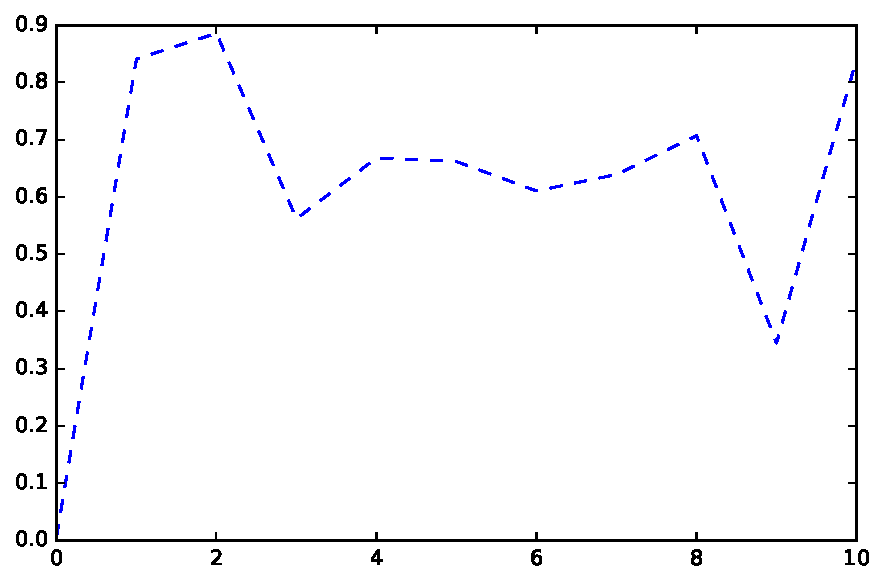
\includegraphics[width=0.5\linewidth]{figures/cnn_diff_slices.pdf} & 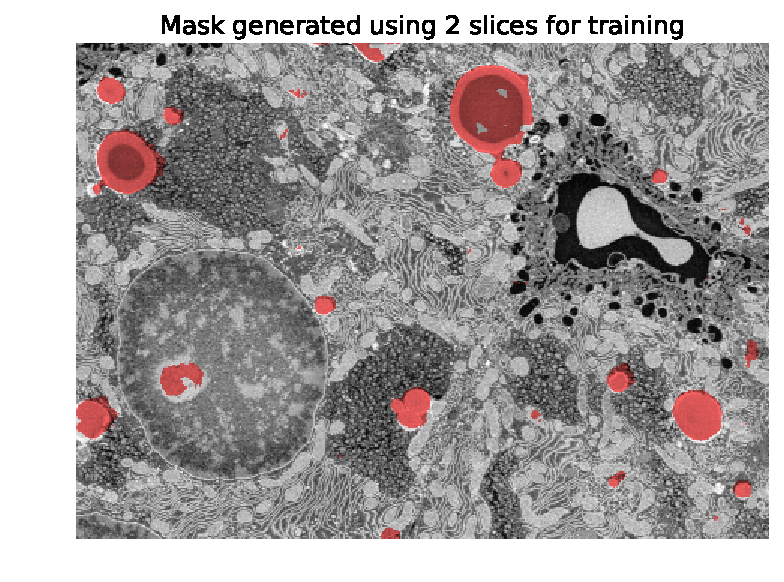
\includegraphics[width=0.5\linewidth]{figures/cnn_mask_2slice.pdf} \\
\end{tabular}
\caption{Left image: F-measure computed for different amount of training data; Right image: Predicted mask for one slice}
\end{figure}
We expected increase in performance with the increase in the amount of data. This does not happen as CNN is not able to converge equivalently for all cases. It is important to remember here that annotating one slice is not same as one object. We can observe these multiple objects in figure 1.2. Also, change in annotation will force us to train network again. These difficulties motivated us to try semi-supervised learning for our task of segmentation.